\documentclass[12pt, letterpaper]{article}
\usepackage[utf8]{inputenc}
\usepackage{graphicx}
\usepackage{indentfirst}
\usepackage{amsmath}
\usepackage{esint}
\usepackage{float}
\usepackage{amssymb}
\usepackage{siunitx}
\graphicspath{ {images/} }

\title{Projeto 1 - F328}
\author{Rian Radeck Santos Costa - 187793 \\ Grupo I06}
\date{07 de Junho de 2022}

\begin{document}

\maketitle 

\newpage

\section{Radiação emitida}
    \par
    A primeira observação que devemos fazer é que enquanto uma partícula carregada está em movimento ela tem um campo fácil de ser observado, como na figura 1.
    
    \begin{figure}[h]
        \centering
        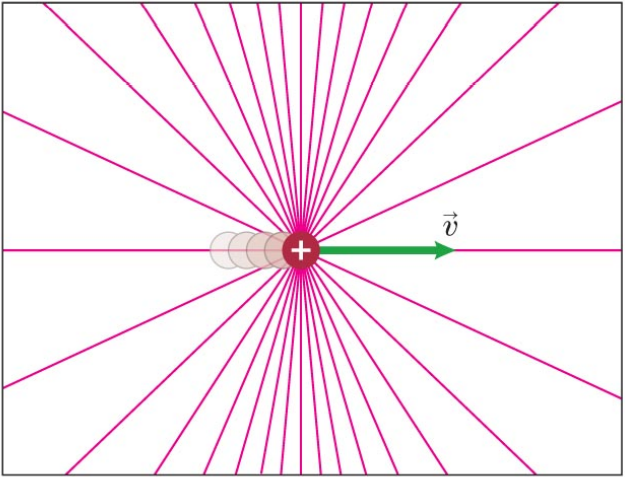
\includegraphics[width=0.4\textwidth]{moving particle}
        \\{Figura 1: Linhas de campo de uma carga com velocidade constante}
        \label{fig:fig1}
    \end{figure}

    Também sabemos que, de acordo com as leis do eletromagnetismo clássico, toda partícula que sofre uma aceleração emite radiação e faz um pulso eletromagnetico no período de aceleração, dividindo o espaço em três regiões, a interna, que já notou que a partícula está se movendo, a externa, que ainda não notou isso e a intermediária, que chamamos de \textit{ring of kinks}.

    \begin{figure}[h]
        \centering
        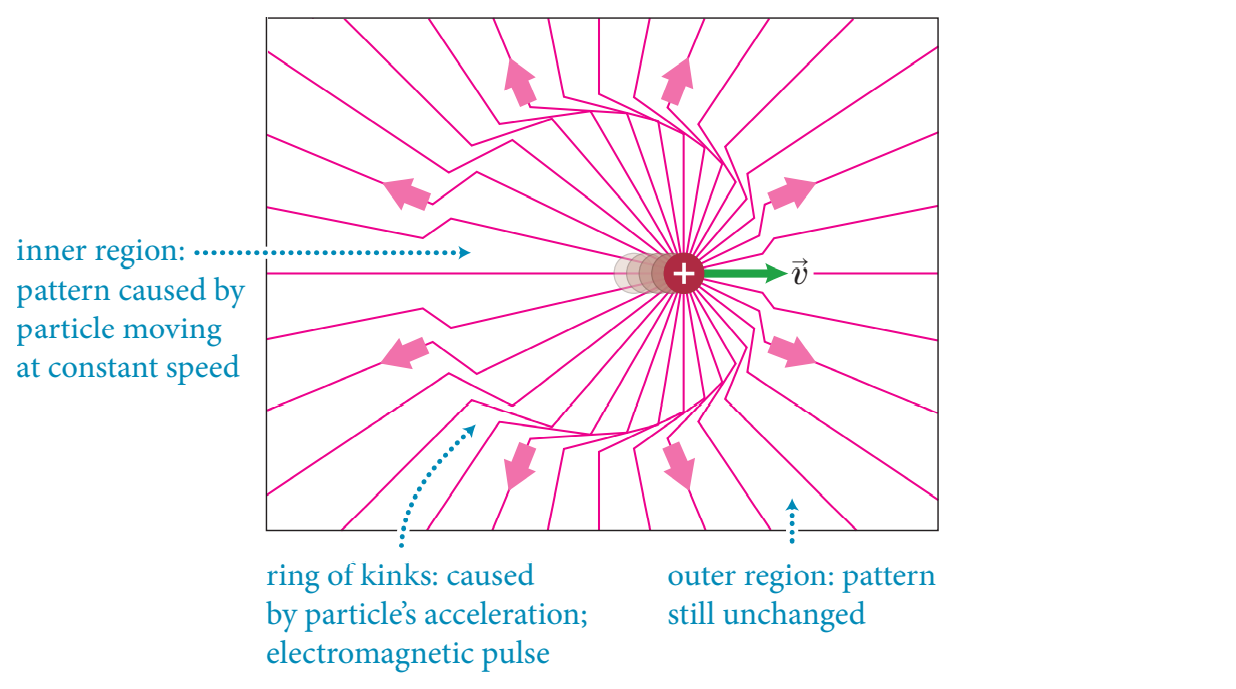
\includegraphics[width=0.7\textwidth]{pulse}
        \\{Figura 2: Partícula carregada que saiu do repouso e mantém velocidade constante}
        \label{fig:fig2}
    \end{figure}

    Vamos então marcar alguns pontos importantes para calcularmos o campo na região intermediária e a potência irradiada. Sabemos que a informação sobre a nossa partícula para qualquer ponto no espaço se move na velocidade da luz, portanto o nosso pulso se move nessa velocidade. Tome um tempo $t = T \gg \tau$, teremos o seguinte diagrama:

    \begin{figure}[h]
        \centering
        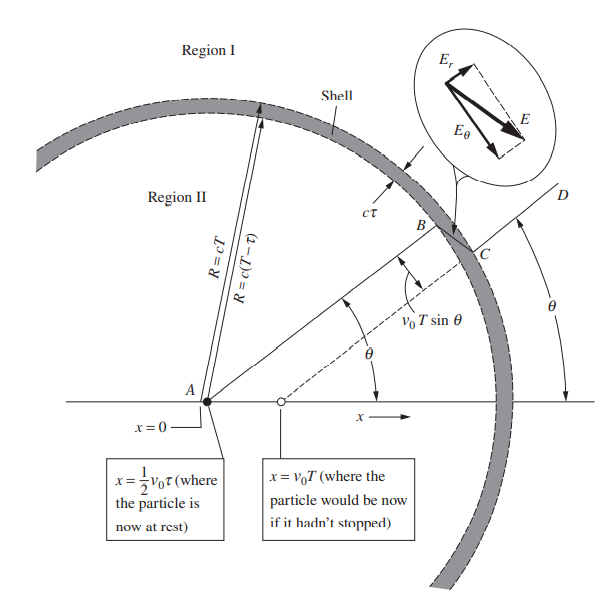
\includegraphics[width=0.8\textwidth]{diagrama}
        \\{Figura 3: Diagrama para um instante $t = T \gg \tau$, um longo tempo após a parada da partícula}
        \label{fig:fig3}
    \end{figure}

    Vamos definir $x = 0$ como o lugar no espaço onde a nossa partícula começou a ser desacelerada e $t = 0$ como o momento que ela começou a ser desacelerada. Definindo esses referenciais, conseguimos definir nossas regiões e a posição onde nossa partícula irá parar, que será definida pela equação de Torricelli $v^2 = v_0 ^2 + 2a\Delta S$. Portanto nossa partícula estará no repouso em $x = \frac{1}{2} v_0 \tau$, já que $a = v_0 /\tau$. Outra posição importante para o nosso diagrama é $x = v_0 T$, que é onde a partícula estaria se nunca tivesse sido desacelerada. Esse ponto é importante pois é onde os pontos no espaço após o pulso eletromagnético pensam que nossa partícula está, já que eles nunca receberam a informação da desaceleração.

    Vamos então definir nossas regiões. Aqui, ``Region I" é a região externa ao pulso, que ainda não recebeu a informação que a partícula parou, ou seja está a uma distância maior que $cT$ do ponto $x = 0$ $(R > cT)$. Similarmente, ``Region II'' é a região que já recebeu essa informação, portanto sua distância ao ponto $x = 0$ é $R \leq c(T - \tau)$ e a região do pulso que está definida no diagrama como ``Shell'' é a que está entre as duas definidas anteriormente e tem espessura de $c\tau$.

    Agora devemos nos perguntar: Qual o formato de uma linha de campo na região de transição? Devemos olhar para a lei de Gaus para obter a resposta. Tome uma linha de campo que sai do ponto A (partícula parada) e atinge o ponto B, no início da região de transição. Essa linha faz uma angulação $\theta$ com o eixo de viagem da partícula. Sabemos então que esse cone de angulação possui uma certa quantidade de fluxo atravessando ele. Se tomarmos um cone que é definido por CD (atinge o eixo de viagem onde a região externa pensa que é onde está a partícula), ele terá o mesmo $\theta$ e, portanto, terá a mesma quantidade de fluxo atravessando-o. (Observe que isso só é verdade pois $v_0$ é pequeno quando comparado a $c$, o que nos deixa ignorar efeitos relativísticos.) Portanto as linhas de campo AB e CD devem estar conectadas por BC, já que são a mesma linha.

    \begin{figure}[H]
        \centering
        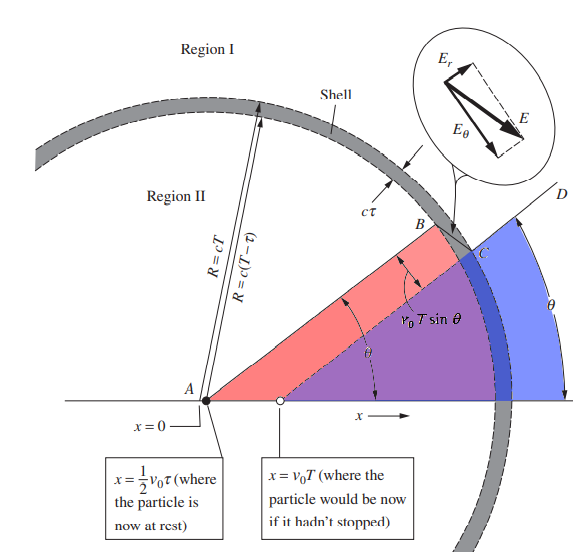
\includegraphics[width=0.65\textwidth]{highlight}
        \\{Figura 4: Cones de fluxo destacados do diagrama.}
        \label{fig:fig4}
    \end{figure}

    Vamos finalmente calcular o valor do campo na região intermediária. Como sabemos a direção do campo, devemos calcular suas componentes $E_r$ (componente radial) e $E_\theta$ (componente transversal). Da geometria do problema podemos concluir que:
    
    \begin{equation} \label{eq1}
    \frac{E_\theta}{E_r} = \frac{v_0 T\sin{\theta}}{c\tau}
    \end{equation}

    Se tomarmos uma gaussiana equivalente a região interna e a casca $(R = cT)$ podemos calcular $E_r$ em B.

    \begin{equation} \label{eq2}
    \begin{split}
        \oiint E_r \delta \vec{A} &= \frac{q_{env}}{\epsilon_0} \\
        E_r(4\pi R^2) &= \frac{q}{\epsilon_0} \\
        E_r &= \frac{q}{4\pi\epsilon_0R^2} \\
        E_r &= \frac{q}{4\pi\epsilon_0c^2T^2} 
    \end{split}
    \end{equation}

    Utilizando o resultado obtido, substituimos na equação \ref{eq1}:

    \begin{equation} \label{eq3}
        E_\theta = \frac{v_0T\sin{\theta}}{c\tau}E_r = \frac{qv_0\sin{\theta}}{4\pi\epsilon_0c^3T\tau}
    \end{equation}

    Mas, $v_0 / \tau = a$ e $cT = R$, então nosso resultado é melhor representado por:

    \begin{equation} \label{eq4}
        E_\theta = \frac{qa\sin{\theta}}{4\pi\epsilon_0c^2R}
    \end{equation}

    Como podemos concluir, $E_\theta$ é proporcional a $1/R$ e, com o passar do tempo, $E_r$ se torna negligível quando comparado a $E_\theta$. Assim, $E$ se torna perpendicular a $R$, o que causa um campo magnético perpenduicular a $E$ e a $R$ com passar de alguns instantes. Isso é uma das propriedades fundamentais de uma onda eletromagnética.

    Vamos então calcular a enrgia que está guardada no campo elétrico transversal, para toda a região intermediária (casca do pulso). A densidade de energia será:

    \begin{equation} \label{eq5}
        \frac{\epsilon_0E_\theta^2}{2} = \frac{q^2a^2\sin^2{\theta}}{32\pi^2\epsilon_0R^2c^4}
    \end{equation}    

    Como o volume da casca será $4\pi R^2 c\tau$ e o valor médio de $\sin^2{\theta}$ sobre uma esfera completa é $\frac{2}{3}$, podemos concluir que a energia total que atravessa o campo elétrico é:

    \begin{equation} \label{eq6}
        \frac{q^2a^2}{32\pi^2\epsilon_0R^2c^4}\frac{2}{3}4\pi R^2c\tau = \frac{q^2a^2\tau}{12\pi\epsilon_0c^3}
    \end{equation}    

    Podemos chegar a mesma conclusão se integrarmos a densidade de energia sobre toda a casca.

    Como descobrimos a energia em relação ao campo elétrico, sabemos que o campo magnético deve ter a mesma quantidade de energia. Assim, a energia total será a soma da energia dos dois campos:

    \begin{equation} \label{eq7}
        \textrm{Energia total propagada pelo campo eletromagnético} =\frac{q^2a^2\tau}{6\pi\epsilon_0c^3}
    \end{equation}

    Perceba que o raio $R$ não participa mais da nossa equação, isso significa que essa quantidade de energia simplesmente passeia pelo espaço, se distanciando da partícula, com a velocidade da luz, a partir do local da desaceleração $(x = 0)$. Como $\tau$ é o período da desaceleração, e também a duração do pulso eletromagnético, podemos declarar que a potência irradiada durante o processo de desaceleração foi:

    \begin{equation} \label{eqMaster}
        P_{rad} = \frac{q^2a^2}{6\pi\epsilon_0c^3}
    \end{equation}

    Perceba também que não importa se nossa partícula está acelerando ou desacelerando, só importa a sua magnitude. Complementando a ideia de diferentes referenciais, $P_{rad}$ é uma grandeza invariante de \textit{Lorentz}, já que $P_{rad}$ é \textit{energia / tempo}, e energia se transforma como o tempo na teoria da relatividade especial.

    Aqui nós obtemos o seguinte resultado: A equação \ref{eqMaster} nos dá a taxa instantânea de irradiação de energia de uma partícula carregada que sofre uma variação de aceleração. Isso é muito útil e pode ser utilizado em diversas aplicações, afinal, ondas eletromagnéticas movem o mundo.

\newpage
\section{Átomo de hidrogênio}

    Aqui vamos trabalhar com o modelo atómico de Rutherford e não o de Bohr, já que Bohr fez correções ao modelo planetário de Rutherford utilizando ideias de teoria quântica de Planck, os conceitos de Einstein sobre o fóton e a mecânica clássica Newtoniana.

    No modelo de Bohr, a sua teoria se aplica da seguinte maneira ao átomo de hidrogênio:

    \begin{enumerate}
        \item O elétron se move em óbitas circulares ao redor do próton, sob a influência de uma força elétrica de atração como na figura 5.
        \item Somente algumas orbitas do elétron são estáveis. Quando em alguma dessas órbitas, o elétron não emite energia na forma de radiação, apesar de estar acelerando (Bohr chamou esses estados de ``estados estacionários''.) Portanto, a quantidade total de energia no átomo permanece a mesma e mecânica clássica pode ser utilizada para descrever a movimentação do elétron. Esse modelo afirma que a aceleração centrípeta do elétron não faz com que ele emita continuamente radiação, perdendo energia e eventualmente espiralando para o núcleo, como previsto para o modelo interplanetário de Rutherford.
        \item O átomo deve emitir radiação somente quando o elétron faz a transição de um estado estacionário mais energético para um estado estacionário menos energético. Essa transição não pode ser visualizada ou tratada classicamente. Em particular, a frequência \textit{f} do fóton emitida na transição de estados está relacionada com a mudança na energia do átomo e não é igual a frequência da movimentação na órbita do elétron. A frequência da radiação emitida é encontrada a partir da expressão da conservação de energia:
        \begin{equation} \label{eq9}
            E_i - E_f = hf
        \end{equation}
        onde $E_i$ é a energia do estado inicial, $E_f$ é a energia do estado final, e $E_i > E_f$. Além disso, a energia de um fóton incidente pode ser absorvida pelo átomo, mas somente se o fóton possuir energia que combina exatamente com a diferença de energia entre um estado permitido do átomo e um estado mais energético. Na sua absorção, o fóton desaparace e o átomo faz uma transição para o estado mais energético.
        \item O tamanho de uma órbita permitida  é determinada pela condição imposta sob o momento angular orbital do elétron: as órbitas permitidas são aquelas para qual o momento angular orbital do elétron sobre o núcleo é quantizado e igual a um múltiplo inteiro de $\hslash = h/2\pi$, onde $h$ é a constante de Planck.

    \end{enumerate}

    \begin{figure}[h]
        \centering
        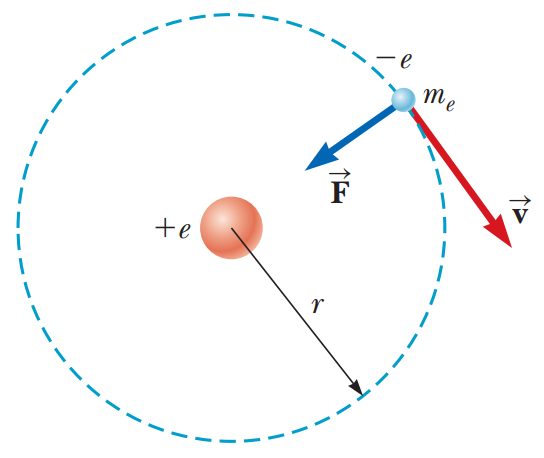
\includegraphics[width=0.5\textwidth]{bohr}
        \\{Figura 5: Modelo do átomo de hidrogênio de Bohr}
        \label{fig:bohr}
    \end{figure}

    O modelo de Bohr foi muito vitorioso com sua concordância com alguns resultados experimentais feitos no átomo de hidrogênio, porém ele sofreu com algumas dificuldades. Uma das primeiras indicações que o modelo de Bohr precisava ser modificado surgiu quando técnicas melhoradas de espectroscopia foram utilizadas para examinar as linhas espectrais do hidrogênio. Surgiram diferenças entre a teoria e os resultados experimentais e esforços para explicar esses e outros devios do modelo de Bohr levaram a modificações na teoria e inevitavelmente a substituição por uma nova.

    \newpage
    Bom, esclarecido o comportamento do átomo de Bohr, vamos então trabalhar com o modelo de Rutherford, que permite raios arbitrários para a órbita do elétron.

    De acordo com a teoria do eletromagnetismo de Maxwell, cargas com aceleração centrípeta com frequência de revolução $f$, devem irradiar ondas eletromagnéticas com frequência $f$, assim o modelo átomico de Rutherford é guiado para autodestruição. 

    \begin{figure}[H]
        \centering
        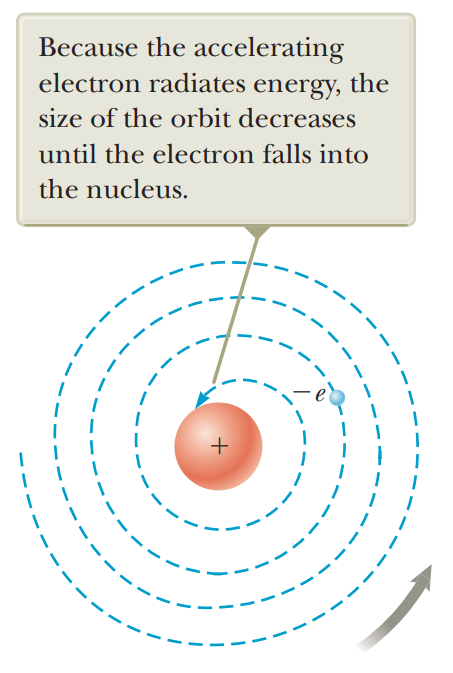
\includegraphics[width=0.5\textwidth]{ruth}
        \\{Figura 6: O modelo átomico de Rutherford prevê seu decaimento}
        \label{fig:ruth}
    \end{figure}

    Considerando o sistema próton-elétron como um sistema não isolado energeticamente, podemos equacionar que:
    \begin{equation} \label{eq10}
        \Delta K + \Delta U = T_{RE}
    \end{equation}
    Onde $K$ é a energia cinética do elétron, $U$ é a energia potencial elétrica do sistema próton-elétron e $T_{RE}$ é a radiação eletromagnética emitida. Como a energia está deixando o sistema, o raio da orbita do elétron diminiu (Figura 6).

    Dessa forma, a medida que o elétron se aproxima do núcleo, a sua velocidade angular aumenta, o que nos leva a uma freqûencia de radiação crescente e o colapso inevitável do átomo.

    Sabemos então que em seu colapso, todo a energia do átomo foi emitida como radiação, portanto utilizando o resultado encontrado na equação \ref{eq7}, teremos a seguinte relação:
    \begin{equation} \label{eq11}
    \begin{split}
        \Delta K + \Delta U &= T_{RE} \\
        \frac{1}{2}m_e v^2 - \frac{e^2}{4\pi\epsilon_0R} &= \frac{e^2a^2\tau}{6\pi\epsilon_0c^3}
    \end{split}
    \end{equation}

    Resolvendo a equação para $\tau$ temos o tempo para o colapso.
    \begin{equation} \label{eq12}
        \tau = \frac{2a_0e^2}{c^3(6\pi\epsilon_0a_0m_e - \frac{e^2}{v_0^2})}
    \end{equation}
    Onde $v_0$, $e$ e $m_e$ são respectivamente a velocidade inicial, a carga e a massa do elétron e $a_0$ é o raio de Bohr.
    Utilizando os valores da seguinte maneira:
    $$
    a_0 = \SI{5.29e-7}{\meter}
    $$$$
    e = \SI{-1.6e-19}{\coulomb}
    $$$$
    c = \SI{2.99e8}{\meter\per\second}
    $$$$
    e_0 = \SI{8.85e-12}{\coulomb\squared\per\newton\per\meter\squared}
    $$$$
    m_e = \SI{9.11e-31}{\kilogram}
    $$$$
    v_0 = 0.75c = \SI{2.24e8}{\meter\per\second}
    $$
    Obtemos que $\tau$, o tempo de colisão será:
    $$
    \tau = \SI{1.26e-23}{\second}
    $$

\newpage
\section{Radiação Síncrotron}

    Seja $v$ a velocidade do elétron no referencial $F$ na terra, vamos calcular então seu campo no referencial $F'$ que é o referencial que se move com o elétron em um dado instante $\delta t$. Usando as transformadas de Lorentz, o campo elétrico em $F'$ será $E' = \gamma v\times B'$, porém $B' = B$, já que no referencial $F'$ a partícula não sente força magnética pois $v' = 0$. 

    Antes de prosseguir com os cálculos, observe que em $F'$
    $$
    \Delta t = \gamma\Delta t' \iff \Delta x' = 0
    $$$$
    E = \gamma E' \iff p' = 0
    $$

    Aqui $E$ representa a energia e não o campo elétrico. Isso implica então que $\Delta E/\Delta t = \Delta E'/\Delta t' \Longrightarrow P = P'$ então, antes de qualquer cálculo, sabemos que nossa radiação emitida será a mesma nos dois referenciais. Vamos então calcular $P'$ em relação ao campo magnético $B$ e as constantes relativísticas.

    Como já descobrimos $E' = \gamma v\times B$, esse campo faz com que a partícula acelere no referencial $F'$, ou seja $v'$ começa a crescer e será diferente de 0 em $F'$ após o instante que estamos analisando. Desenvolvendo a equação $F = m_ea \Rightarrow eE' = m_ea \Rightarrow a = eE'/m_e$, obtemos a aceleração do elétron. Utilizando o resultado da equação \ref{eqMaster}, essa aceleração causa uma irradiação no elétron a uma taxa de
    \begin{equation} \label{eq13}
        P' = \frac{q^2a^2}{6\pi\epsilon_0c^3} = \frac{e^2(eE'/m_e)^2}{6\pi\epsilon_0c^3} = \frac{e^4\gamma^2v^2B^2}{6\pi\epsilon_0c^3m_e^2} \approx \frac{e^4\gamma^2B^2}{6\pi\epsilon_0m_e^2c}
    \end{equation}
    e a aproximação final foi feita devido ao fato de nosso elétron ser altamente relativístico.

    Veja que após o instante de tempo $\delta t$ devemos escolher um novo referencial $F''$ que o elétron esteja parado ($v'' = 0$), já que ele está em constante processo de aceleração ($v' \neq 0$ após um $\delta t$), um instante após o outro.


\end{document}